%!TEX program = xelatex
\documentclass[12pt,a4paper]{article}%titlepage表示标题单独页
\usepackage{ctex}%ctex套用英文标题格式(建议在英文论文混排中文时使用),ctexcap套用中文格式(等同于\documentclass{ctexart})
\renewcommand{\figurename}{图}
\renewcommand{\tablename}{表}
\renewcommand{\contentsname}{目录}
%\renewcommand{\thefigure}{\chinese{figure}}%将图片计数改为汉字数字
%\renewcommand{\thetable}{\chinese{table}}%将表格计数改为汉字数字
\usepackage[top=0.75in,bottom=0.75in,left=0.75in,right=0.75in]{geometry}%页边距设置:数据来自MS word的默认值
\usepackage[CJKbookmarks]{hyperref}%给pdf文档添加互动式链接和书签

\usepackage{amsmath,amssymb,esint,mathrsfs}%数学公式类宏包;最末为积分符号拓展
\allowdisplaybreaks[0]%允许多行公式间换页,用//*表示不允许换页
\numberwithin{equation}{section}%公式编号包含章节
\usepackage{bm}%加粗(用于vector)
%\usepackage{textcomp}%符号包,不能用于数学模式,建议不要和SIunits混用
%\usepackage[squaren]{SIunits}%科学单位包,可以用于数学模式(为了统一不要和textcomp混用),squaren选项消除和amssymb的冲突
\usepackage{graphicx}%插图宏包
%\usepackage{picinpar}%图文绕排
\usepackage{array}%表格宏包
%\usepackage{longtable}%长表格宏包
\usepackage{multirow}%多行合并的表格宏包
%\usepackage{booktabs}%表格线宏包
\usepackage{extarrows}

%\usepackage[basic,box,gate,oldgate,ic,optics,physics]{circ}%电路图宏包
%\usepackage[normalem]{ulem}%下划线,删除线等宏包,参数表示不修改\emph{}格式
%\usepackage[version=3]{mhchem} %\ce{.}输入化学式
%\usepackage{mychemistry}%化学宏包,包含mhchem和chemfig
%\usepackage[symbol]{footmisc}%脚注拓展,选项表示用符号做脚注记号

\renewcommand*{\vec}[1]{\bm{#1}}%矢量的格式,这里是加粗
\newcommand{\dif}{\,\mathrm d}
\newcommand\mi{\mathrm{i}}
\newcommand\e{\mathrm{e}}%定义数学模式中常用的正体字符
\newcommand*{\uvec}[1]{\hat{\vec{#1}}}
\newcommand\dbar{\ensuremath{\,\mathchar"AF\mkern-12mu \mathrm{d}}}
\renewcommand*{\Re}{\operatorname{Re}}
%-------------
% 考完之后再次使用记得调整相对论的符号系统
%-------------
\begin{document}
\title{电动力学整理}
\author{吕铭 Lyu Ming}
\maketitle
\tableofcontents

如未特别说明, 以下相关公式均使用 Einstein 求和规则
\section{数学准备} % (fold)
\label{sec:math_prep}
\begin{enumerate}
    \item 各向同性张量: $T'_{i_1,i_2,\cdots,i_n} = T_{i_1,i_2,\cdots,i_n}$:
    \begin{itemize}
        \item 零阶张量是各向同性的
        \item 一阶张量除零矢量外, 都\emph{不是}各向同性的
        \item 二阶张量中各向同性张量必为 $\lambda \delta_{ij}$
        \item 三阶张量中各向同性张量必为 $\lambda \epsilon_{ijk}$
        \item 四阶张量中各向同性张量必为 $\lambda\delta_{ij}\delta_{kl} + \alpha\delta_{ik}\delta_{jl} + \beta\delta_{il}\delta_{jk}$
    \end{itemize} 
    \item 场的积分
    \begin{align}
        &\int_A^B\dif\vec l\cdot\nabla\varphi = \varphi(B) - \varphi(A) \\
        &\int_V\dif \tau\lambda\cdot\vec f = \oint_{\partial V}\dif\vec S\cdot\vec f \\
        &\int_S\dif\vec S\cdot\nabla\times\vec f = \oint_{\partial S}\dif\vec l \cdot\vec f \\
        &\int_S\dif \vec S\times\nabla = \oint_{\partial S}\dif\vec l
    \end{align}
    \item 曲线坐标\footnote{注意在计算 $\nabla\cdot f$ 和 $\nabla\cdot f$ 中基矢量随着角度的变化. }
    \begin{itemize}
        \item 柱坐标
        \begin{align}
            &\nabla = \uvec e_r\frac{\partial}{\partial r} + \uvec e_\theta\frac 1r\frac{\partial}{\partial\theta} + \uvec e_z\frac{\partial}{\partial z} \\
            &\nabla^2 = \frac 1r\frac{\partial}{\partial r}\left( r\frac{\partial}{\partial r} \right) + \frac 1{r^2}\frac{\partial^2}{\partial \theta^2} + \frac{\partial^2}{\partial z^2}
        \end{align} 
        \item 球坐标
        \begin{align}
            &\nabla = \uvec e_r\frac{\partial}{\partial r} + \uvec e_\theta\frac 1r\frac{\partial}{\partial \theta} + \uvec e_\varphi\frac1{r\sin\theta}\frac{\partial}{\partial\varphi} \\
            &\nabla^2 = \frac 1{r^2}\frac{\partial}{\partial r}\left(r^2\frac{\partial}{\partial r}\right) + \frac1{r^2\sin\theta}\frac{\partial}{\partial\theta}\left(\sin\theta\frac{\partial}{\partial\theta}\right) + \frac 1{r^2\sin\theta}\frac{\partial^2}{\partial\varphi^2}
        \end{align}
    \end{itemize}
    \item $\delta$ 函数
    \begin{align}
        &\delta(f(x)) = \sum_{f(x_i) = 0}\frac 1{|f'(x_i)|}\delta(x-x_i) \\
        &\delta(\vec r - \vec r') = -\frac 1{4\pi}\nabla^2\frac 1{|\vec r-\vec r'|} \\
        &\partial_i\partial_j\frac1{|\vec r- \vec r'|} = -\frac{\delta_{ij}}{|\vec r - \vec r'|^3} + 3\frac{(r_i-r'_i)(r_j - r'_j)}{|\vec r - \vec r'|^5} - \frac {4\pi}3\delta_{ij}\delta(\vec r - \vec r')
    \end{align}
    \item Helmholtz 定理
    \begin{align}
        \vec F(\vec r) &= \underbrace{-\nabla U(\vec r)}_{\mbox{\footnotesize 横场}} + \underbrace{\nabla\times\vec W(\vec r)}_{\mbox{\footnotesize 纵场}} + \mbox{边界项} \\
        U(\vec r) &= \int\dif \tau'\frac{\nabla'\cdot \vec F(\vec r')}{4\pi|\vec r - \vec r'|} \\
        \vec W(\vec r) &= \int\dif \tau'\frac{\nabla'\times \vec F(\vec r')}{4\pi|\vec r - \vec r'|} 
    \end{align}
    纵场和横场正交
    \begin{equation}
        \int\dif \tau'(-\nabla U)\cdot(\nabla\times \vec W) = 0
    \end{equation}
\end{enumerate}
% section math_prep (end)

\section{电磁场的普遍方程} % (fold)
\label{sec:general_equ_for_EMF}
Maxwell 方程
\begin{align}
    &\oint_{\partial V}\vec D\cdot \dif \vec S = \int_V \rho \dif \tau &
    &\nabla\cdot\vec D = \rho \\
    &\oint_{\partial V} \vec B\cdot \dif \vec S = 0 &
    &\nabla\cdot\vec B = 0 \\
    &\oint_{\partial S}\vec E\cdot\dif\vec l = -\int_S\frac{\partial \vec B}{\partial t}\cdot\dif\vec S &
    &\nabla\times\vec E = -\frac{\partial \vec B}{\partial t} \\
    &\oint_{\partial S}\vec H\cdot\dif\vec l = \int_S\left(\vec j + \frac{\partial\vec D}{\partial t}\right)\cdot\dif\vec S &
    &\nabla\times\vec H = \vec j + \frac{\partial\vec D}{\partial t}
\end{align} 
边值关系
\begin{align}
    &\uvec n\times(\vec E_2 -\vec E_1) = 0 \\
    &\uvec n\times(\vec H_2 - \vec H_1) = \vec\alpha \\
    &\uvec n\cdot(\vec D_2 - \vec D_1) = \sigma \\
    &\uvec n \cdot(\vec B_2 - \vec B_1) = 0
\end{align}
\subsection{介质关系} % (fold)
\label{sub:medium}
电位移与磁场强度
\begin{align}
    \vec D &= \varepsilon_0\vec E + \vec P & \vec H &= \vec B/\mu_0 - \vec M
\end{align}
\begin{enumerate}
    \item 电极化强度 $\vec P$ 与感应电荷
    \begin{align}
        \rho_{\mathrm P} &= -\nabla\cdot\vec P & \vec j_{\mathrm P} &= \frac{\partial \vec P}{\partial t} & \sigma_{\mathrm P} &= -\uvec n\cdot(\vec P_2 - \vec P_1)
    \end{align}
    \item 磁化强度 $\vec M$ 与感应电流
    \begin{align}
        \vec j_{\mathrm M} &= \nabla\times\vec M & \vec \alpha_{\mathrm M} = \uvec n\times(\vec M_2 - \vec M_1)
    \end{align}
    \item 线性介质与极化率 $\chi_{\mathrm e}$, 磁化率 $\chi_{\mathrm M}$
    \begin{align}
        \vec D &= \varepsilon_0(1+\chi_{\mathrm e})\vec E = \varepsilon \vec E & \vec B &= \mu_0(1+\chi_{\mathrm M})\vec H = \mu\vec H
    \end{align}
    \begin{itemize}
        \item 顺磁介质 ($\mu_r> 1$)
        \item 抗磁介质 ($\mu_r<1$) 
        \item 铁磁介质 (具有磁滞回线, 永磁材料, 软磁体, 磁记录材料)
        \item 磁电极化介质 (电场驱动磁化与磁场驱动极化)
    \end{itemize}
\end{enumerate}
导体与欧姆定律 $\vec j = \gamma\vec E = \vec E/\lambda$
% subsection medium (end)
\subsection{势与规范变换} % (fold)
\label{sub:potential}
通过 $\nabla\cdot\vec B = 0$ 与 $\nabla\times\vec E$ 定义
\begin{align}
    \vec E &= -\nabla\varphi - \frac{\partial\vec A}{\partial t} &
    \vec B &= \nabla\times\vec A
\end{align}
\begin{enumerate}
    \item (真空中的) d'Alembert 方程, 与 Maxwell 方程组等价
    \begin{align}
        &\nabla^2\vec A - \frac 1{c^2}\frac{\partial^2\vec A}{\partial t^2} - \nabla\left(\nabla\cdot\vec A + \frac 1{c^2}\frac{\partial \varphi}{\partial t}\right) = -\mu_0\vec j \\
        &\nabla^2\varphi - \frac{\partial}{\partial t}\nabla\cdot\vec A = -\frac{\rho}{\varepsilon_0}
    \end{align}
    \item 规范变换
    \begin{align}
     \vec A &\rightarrow \vec A + \nabla\chi 
     &\varphi &\rightarrow \varphi - \frac{\partial\chi}{\partial t}
    \end{align}
    \item Coulomb 规范
    \begin{equation}
        \nabla\cdot\vec A = 0\Longrightarrow 
        \nabla\vec A - \frac 1{c^2}\frac{\partial^2\vec A}{\partial t^2} = -\mu_0\vec j + \frac 1{c^2}\frac{\partial}{\partial t}\nabla\varphi \equiv -\mu_0\vec j^* \quad
        \nabla^2\varphi = -\frac{\rho}{\varepsilon_0}
    \end{equation}
    \item Lorenz 规范
    \begin{equation}
        \nabla\cdot\vec A + \frac 1{c^2}\frac{\partial \varphi}{\partial t} = 0\Longrightarrow
        \nabla^2\vec A - \frac 1{c^2}\frac{\partial^2\vec A}{\partial t^2} = -\mu_0\vec j \quad
        \nabla^2\varphi - \frac 1{c^2}\frac{\partial^2\varphi}{\partial t^2} = -\frac{\rho}{\varepsilon_0}
    \end{equation}
\end{enumerate}
% subsection potential (end)
\subsection{电荷运动学与动力学关系} % (fold)
\label{sub:dynamics}
\begin{enumerate}
    \item 洛伦兹力
    \begin{equation}    
        \vec f = \rho\vec E + \vec j \times \vec B
    \end{equation}
    \item 电荷守恒
    \begin{equation}
        \nabla\cdot\vec j + \frac{\partial\rho}{\partial t} = 0
    \end{equation}
    \item 能流密度与能流密度 (Poynting 矢量)
    \begin{align}
        w &= \int(\vec E\cdot\dbar\vec D + \vec H\cdot\dbar\vec B) \stackrel{\mbox{\footnotesize 线性}}{=\joinrel=\joinrel=} \frac 12 (\vec E\cdot\vec D + \vec H\cdot\vec B) &
        \vec S &= \vec E\times\vec H \label{equ:energy_density_and_flux}
    \end{align}
    能量守恒
    \begin{equation}
        \nabla\cdot\vec S + \frac{\partial w}{\partial t} + \vec f\cdot\vec v = 0
    \end{equation}
    \item (真空中的) 动量密度与动量流密度
    \begin{align}
        \vec g &= \varepsilon_0\vec E \times \vec B = \varepsilon_0\mu_0\vec S 
        = \frac{\vec S}{c^2} \label{equ:momentum_density}\\
        \mathcal J_{ij} &= -\varepsilon_0 E_iE_j - \frac 1{\mu_0}B_i B_j + \frac 12 \delta_{ij}\left(\varepsilon_0\vec E^2 + \frac 1{\mu_0}\vec B^2\right) \label{equ:momentum_density_flux}\\
        &= -\varepsilon_0 E_iE_j - \frac 1{\mu_0}B_i B_j + \delta_{ij} w
    \end{align}
    动量守恒
    \begin{equation}
        \partial_j\mathcal J_{ij} +\frac{\partial g_i}{\partial t} + f_i = 0
    \end{equation}
    一般的带电体间牛顿第三运动定律未必成立
\end{enumerate}
% subsection dynamics (end)
% section general_equ_for_EMF (end)

\section{静场与稳恒电流} % (fold)
\label{sec:static_field}
\subsection{静电场} % (fold)
\label{sub:static_elctro}
\begin{enumerate}
    \item 库伦规范下的均匀介质:
    \begin{align}
        \nabla^2\varphi &= -\frac{\rho}{\varepsilon} &\nabla^2\vec A = -\mu\vec j
    \end{align}
    \item 非极值定理: 均匀介质中无电荷分布的区域内的任何一点的静电势都不可能取极值. 静电势极值只能位于边界或有电荷处.
    \item 唯一性定理: 分区连续介质内电荷分布已知, 且如下边界条件满足其一
    \begin{align}
        \varphi|_{S_i} &\mbox{已知} &\left.\frac{\partial\varphi}{\partial\uvec n}\right|_{S_i} &\mbox{已知}
    \end{align}
    则静电场唯一确定
    \item 导体的唯一性定理: 即边界条件增加一条
    \begin{equation}
        \varphi|_{S_i} = \mbox{const.} \land \oint_{S_i}\varepsilon\frac{\partial\varphi}{\partial\uvec n}\dif S = Q_i\mbox{ 已知}
    \end{equation}
    \item 分离变量法: 求 Laplace 方程的解
    \begin{enumerate}
        \item 球坐标下: 
        \begin{equation}
            \varphi(r,\theta,\phi) = \sum_{n,m}\mathrm P_n^m(\cos\theta)\left[\left(a_{nm}r^n + \frac{b_{nm}}{r^{n+1}}\right)\cos m\phi + \left(c_{nm}r^n + \frac{d_{nm}}{r^{n+1}}\right)\sin m\phi\right]
        \end{equation}
        \item 关于 $z$ 轴对称的情形
        \begin{equation}
            \varphi(r,\theta) = \sum_n\left(a_n r^n + \frac{b_n}{r^{n+1}}\right)\mathrm P_n(\cos\theta)
        \end{equation}
        其中 $m\in\mathbb N$ 来自于 $\phi$ 坐标的周期性, $n\in\mathbb N$ 来自于 $\theta = \pi$ 处的非奇异. \\
        其他情况详见数理方程
        \item 柱坐标下
        \begin{align}
            \varphi(r,\theta,z) &= A_0\ln r + (A_0'\ln r + B_0)\theta + C_0 + \sum_n(A_n r^n + B_n r^{-n})\cos(n\theta + \alpha_n) \\
            & \quad + \sum_{k\neq 0,n}D_n\mathrm J_n(kr)\sinh(kz)\cos(n\theta + \alpha_n)
        \end{align}
        最后一项在二维情形下消失
        \item 关于 Legendre 函数
        \begin{itemize}
            \item 正交性
            \begin{equation}
                \int_{-1}^1\mathrm P_m(x)\mathrm P_n(x)\dif x = \frac2{2n+1}\delta_{mn}
            \end{equation}
            \item 完备性
            \begin{equation}
                \sum_{n=0}^\infty \mathrm P_n(x) \mathrm P_n(x') = \frac{2}{2n+1}\delta(x-x')
            \end{equation}
            \item 生成函数
            \begin{equation}
                \frac 1{|\vec r - \vec r'|} = (r^2 + r'^2 - 2rr'\cos\gamma)^{-1/2} = \sum_{n=0}^\infty\frac{r^n_<}{r^{n+1}_>}\mathrm P_n(\cos\gamma)
            \end{equation}
            \item 微分计算公式
            \begin{equation}
                \mathrm P_n = \frac1{2^n n!}\frac{\dif^n}{\dif x^n}(x^2 - 1)^n
            \end{equation}
        \end{itemize}
        \item 球谐函数 (spherical harmonics)
        \begin{equation}
            \mathrm Y_{l}^m(\theta,\phi) = \sqrt{\frac{2l+1}{4\pi}\frac{(l-m)!}{(l+m)!}}\mathrm P_l^m(\cos\theta)\e^{\mi m\phi}
        \end{equation}
    \end{enumerate}
    \item 镜象法
    \item Green 函数
    \begin{equation}
        \nabla^2 G(\vec r, \vec r') = -\frac 1\varepsilon\delta(\vec r - \vec r')
    \end{equation}
    \begin{enumerate}
        \item $\varphi|_{S}$ 已知, 取 $G(\vec r',\vec r)|_{\vec r'\in S} = 0$
        \begin{equation}
            \varphi (\vec r) = \int_V\dif \tau'\rho(\vec r')G(\vec r',\vec r) - \varepsilon\oint_S\dif S'\varphi(\vec r')\frac{\partial G(\vec r',\vec r)}{\partial \uvec n'}
        \end{equation}
        \item $\left.\frac{\partial \varphi}{\partial \uvec n}\right|_{S}$ 已知, 取 $\left.\frac{\partial G(\vec r',\vec r)}{\partial \uvec n'}\right|_{\vec r'\in S} = -\frac 1{\varepsilon S}$
        \begin{equation}
            \varphi(\vec r) = \int_V\dif \tau\rho(\vec r')G(\vec r', \vec r) + \varepsilon\oint_S\dif S' G(\vec r', \vec r)\frac{\partial \varphi(\vec r')}{\partial \uvec n'} + \langle\varphi(S) \rangle
        \end{equation}
        \item 无界空间, 自然边界条件
        \begin{equation}
            \varphi(\vec r) = \int_V\dif \tau\rho(\vec r')G(\vec r', \vec r)
        \end{equation}
    \end{enumerate}
    \item 静电势能与电场能
    \begin{equation}
        W = \frac 12\int\dif \tau\vec E\cdot \vec D = -\frac 12\oint\dif\vec S\cdot\varphi\vec D + \frac 12 \int\dif \tau\rho\varphi = \frac 12\int\dif \tau\rho\varphi
    \end{equation}
    对于线性介质
    \begin{equation}
     W = \frac 1{8\pi\varepsilon}\iint\dif \tau\dif \tau' \frac{\rho(\vec r)\rho(\vec r')}{|\vec r -\vec r'|}
    \end{equation}
    $\rho = \rho_1 + \rho_2$, 则 $W = W_1 + W_2 + W_{\mathrm{int}}$
    \begin{equation}
        W_{\mathrm{int}} = \int\dif \tau\rho_1\varphi_2 = \int\dif \tau\rho_2\varphi_1
    \end{equation}
    即为静电势能, 静电势能是电场能的唯象表述
    \item Thomson 定理: 电荷在不接地的导体上的静态分布恒使静电能取极小值
\end{enumerate}
% subsection static_elctro (end)
\subsection{静磁场} % (fold)
\label{sub:static_mag}
\begin{enumerate}
    \item 稳恒电流与静电场满足相似的方程
    \item 磁场能
    \begin{equation}
        W = \frac 12\int\dif \tau\vec B\cdot\vec H = \frac 12\oint\dif\vec S\cdot(\vec A\times\vec H) + \frac 12\int\dif \tau\vec A\cdot\vec j = \frac 12\int\dif \tau\vec A\cdot\vec j
    \end{equation}
    线性介质
    \begin{equation}
        W = \frac{\mu}{8\pi}\iint\dif \tau\dif \tau'\frac{\vec j(\vec r)\cdot\vec j(\vec r')}{|\vec r - \vec r'|}
    \end{equation}
    类似的可以定义磁势能
    \begin{equation}
        W_{\mathrm{int}} = \int\dif \tau\vec j \cdot \vec A
    \end{equation}
    \item 磁场的一般解法: 
    \begin{itemize}
        \item 一般的直接对照电场解法
        \item 剩磁: $\vec B = \mu_1\vec H + \mu_0 \vec M_0$, 
        \begin{align}
            \nabla\cdot(\mu\vec H) &= -\nabla\cdot(\mu_0\vec M_0) \\
            \nabla\times\vec H &= 0
        \end{align}
        \item 有传导电流
        \begin{align}
            \nabla\times\vec H &= \vec j &
            \nabla\cdot\vec B &= 0
        \end{align}
        Biot-Savart 定律
        \begin{equation}
            \vec B = \int\dif \tau \frac{\mu\vec j \times (\vec r - \vec r')}{4\pi|\vec r - \vec r'|^3}
        \end{equation}
    \end{itemize}
\end{enumerate}
% subsection static_mag (end)
\subsection{多极展开} % (fold)
\label{sub:multipolar_expansion}
\begin{enumerate}
    \item 电势
    \begin{equation}\label{equ:multipole_for_phi}
        \varphi = \sum_{n=0}^\infty \frac 1{4\pi\varepsilon}\frac{(-)^n}{n!}\left(\frac{\partial}{\partial x_{i_1}}\frac{\partial}{\partial x_{i_2}}\cdots\frac{\partial}{\partial x_{i_n}}\frac 1 r\right)q_{i_1,i_2,\cdots,i_n}
    \end{equation} 
    \begin{itemize}
        \item 电多极矩
        \begin{equation}
            q_{i_1,i_2,\cdots,i_n} = \int\dif \tau' \rho(\vec r')\prod_{k=1}^n x'_{i_k}
        \end{equation}
        \item 能量, 力, 力矩
        \begin{align}
            W &= Q\varphi(\vec r) + \sum_{n=1}^\infty \left[-\frac 1{n!}q_{i_1,i_2,\cdots,i_n}\left(\left.\frac{\partial}{\partial x'_{i_2}}\frac{\partial}{\partial x'_{i_3}}\cdots\frac{\partial}{\partial x'_{i_n}} E_{i_1}(\vec r')\right|_{\vec r' = \vec r}\right)\right] \\
            \vec F &= Q\vec E(\vec r) + \sum_{n=1}^\infty \frac 1{n!}q_{i_1,i_2,\cdots,i_n}\left(\left.\frac{\partial}{\partial x'_{i_1}}\frac{\partial}{\partial x'_{i_2}}\cdots\frac{\partial}{\partial x'_{i_n}} \vec E(\vec r')\right|_{\vec r' = \vec r}\right) \\
            \vec L &= \sum_{n=0}^\infty \frac 1{n!} \epsilon_{ijk}q_{i,i_1,i_2,\cdots,i_n}\uvec e_k \left(\left.\frac{\partial}{\partial x'_{i_1}}\frac{\partial}{\partial x'_{i_2}}\cdots\frac{\partial}{\partial x'_{i_n}} E_j(\vec r')\right|_{\vec r' = \vec r}\right) 
        \end{align}
        \item 电偶极矩 
        \begin{align}
            \varphi_1 &= \frac{\vec r\cdot\vec p}{4\pi\varepsilon r^3} \\
            \vec E_1 &= \frac 1{4\pi\varepsilon}\left[-\frac{\vec p}{r^3} + \frac{3\vec r(\vec p\cdot\vec r)}{r^5}\right] - \frac{\vec p}{3\varepsilon}\delta(\vec r) \\
            W_1 &= -\vec p\cdot\vec E
        \end{align}
        \item 电四极矩的补充定义
        \begin{equation}\label{equ:elctro_quadrupole}
            \mathscr D_{ij} = \int\dif \tau'(3x'_ix'_j - r'^2\delta_{ij})\rho(\vec r')
        \end{equation}
        于是有 $\mathscr D_{ii} = 0$
    \end{itemize}
    \item 磁矢量势
    \begin{equation}\label{equ:multipole_for_A}
        \vec A(\vec r) = \sum_{n=1}^\infty \frac{\mu}{4\pi}\frac{(-)^n}{n!}\left(\frac{\partial}{\partial x_{i_1}}\frac{\partial}{\partial x_{i_2}}\cdots\frac{\partial}{\partial x_{i_n}}\frac 1 r\right)\vec J_{i_1,i_2,\cdots,i_n}
    \end{equation}
    零阶项是 $0$
    \begin{itemize}
        \item 磁多极矩 
        \begin{equation}\label{equ:mag_multipole}
            \vec J_{i_1,i_2,\cdots,i_n} = \int\dif \tau'\vec j(\vec r')\prod_{k=1}^n x'_{i_k}\qquad (\vec J = 0)
        \end{equation}
        \item 磁偶极矩与磁矩
        \begin{align}
            \vec m &= \frac 12\int_V\dif \tau'\vec r'\times\vec j \qquad\left(=\frac 12\sum_i\frac{q_i}{M_i}\vec L_i\right) \label{equ:mag_dipole}\\
            \vec A_1 &= \frac{\mu}{4\pi}\vec m\times\frac{\vec r}{r^3} \\
            \vec B_1 &= \frac{\mu}{4\pi}\left(-\frac{\vec m}{r^3} + \frac{3\vec r(\vec m\cdot\vec r)}{r^5}\right)
        \end{align}
        特别的, 对于电流圈
        \begin{equation}
            \vec m = I\int\dif\vec S = I\vec S
        \end{equation}
    \end{itemize}
\end{enumerate}
% subsection multipolar_expansion (end)
% section static_field (end)

\section{电磁波} % (fold)
\label{sec:EMW}
以下 $\vec X \in \{\vec E, \vec B\}$
\subsection{定态电磁波解} % (fold)
\label{sub:stationary_state}

\begin{enumerate}
    \item 均匀绝缘介质中, 无自由电荷的波动方程
    \begin{equation}
        \nabla^2 \vec X - \mu\varepsilon\frac{\partial^2\vec X}{\partial t^2} = 0
    \end{equation} 
    \item 均匀绝缘介质中的平面波解 $\vec X (\vec r, t) = \vec X (t - \uvec n\cdot \vec r / v)$, $v = 1/\sqrt{\mu\varepsilon}$: 
    \begin{align}
        &\frac{\partial}{\partial t}(v\vec B - \uvec n\times\vec E) =  0 & 
        \frac{\partial}{\partial t}(\uvec n\cdot\vec E) = 0\\
        &\frac{\partial}{\partial t}(\vec v\times \vec B + \vec E) = 0 &
        \frac{\partial}{\partial t}(\uvec n\cdot\vec B) = 0
    \end{align}
    略去时间无关项, 则$E = vB$, $w_{\mathrm e} = w_{\mathrm m}$, $\vec S = \vec v (w_{\mathrm e} + w_{\mathrm m})$
    \item 定态电磁波 $\vec X(\vec r,t) = \vec X(\vec r)\e^{-\mi\omega t}$. 
    \begin{itemize}
        \item 均匀介质中的定态电磁波
        \begin{align}
            (\nabla^2 + k^2)\vec X &= 0 & \nabla\cdot\vec X&= 0
        \end{align}
        其中 $k^2 = \omega^2\mu\varepsilon + \mi\omega\mu\gamma$. 电磁场关系
        \begin{align}
            \vec B &= -\frac\mi\omega\nabla\times\vec E & \vec E &= \frac1{\mu(\gamma-\mi\omega\varepsilon)}\nabla\times\vec B
        \end{align}
        \item 平面波解
        \begin{equation}
            \vec X = \tilde{\vec X_0}\e^{\mi(\vec k\cdot\vec r - \omega t)} = \uvec e_i |X_{0i}|\e^{-\vec k_{\mathrm I}\cdot\vec r}\e^{\mi(\vec k_{\mathrm R}\cdot\vec r - \omega t)}
        \end{equation}
        \begin{itemize}
            \item 复振幅关系
            \begin{align}
                &\vec k \cdot\vec B_0 = 0 
                && \vec k \cdot\vec E_0 = 0\\
                &\vec B_0 = \frac{\vec k}\omega \times \vec E_0 
                && \vec E_0 = \frac{\vec k}{\mu\gamma-\mi\omega\mu\varepsilon}\times\vec B_0
            \end{align}
            ($\vec k_{\mathrm I} \neq 0$ 时右手关系不成立, 复振幅不能很好的定义夹角)
            \item 相速度 $v_\phi = \omega\vec k_{\mathrm R}/k_{\mathrm R}^2$
            \item 沿着传播方向总是衰减的 $\vec k_{\mathrm R}\cdot\vec k_{\mathrm I} = \frac 12 \omega\mu\gamma > 0$
            \item 穿透深度 $\delta = 1/(\vec k_{\mathrm I}\cdot\vec k_{\mathrm R}/k_{\mathrm R}) = 2k_{\mathrm R}/\omega\mu\gamma$
            \item 能量密度, 能流密度
            \begin{align}
                \langle w_{\mathrm e} \rangle &= \left\langle \frac 12\varepsilon \vec E_{\mathrm R}^2\right\rangle = \frac 14\varepsilon\Re[\vec E\cdot\vec E^*] = \frac 14\varepsilon\Vert\vec E\Vert^2\\
                \langle w_{\mathrm m} \rangle &= \left\langle \frac 1{2\mu}\vec B_{\mathrm R}^2\right\rangle = \frac 1{4\mu}\Vert\vec B\Vert^2 \\
                &= \frac 1{4\mu\omega^2}\left[\Vert\vec k\Vert^2\Vert\vec E\Vert^2 - |\vec k\cdot\vec E^*|^2\right]\\
                \langle\vec S \rangle &= \left \langle\frac 1\mu\vec E_{\mathrm R}\times\vec B_{\mathrm R}\right \rangle = \frac 1{2\mu}\Re[\vec E\times\vec B^*]\\
                &= \frac 1{2\mu\omega}\Re[\Vert\vec E\Vert^2\vec k-(\vec k\cdot\vec E^*)\vec E]
            \end{align}
            绝缘体 $\vec k = \vec k^*, \vec k\cdot\vec E = 0\Rightarrow \langle w_{\mathrm e} \rangle = \langle w_{\mathrm m} \rangle$
        \end{itemize}
    \end{itemize}
\end{enumerate}
% subsection stationary_state (end)
\subsection{电磁波的反射与折射} % (fold)
\label{sub:reflect_and_refraction}
    \begin{figure}[hbt]
        \centering
        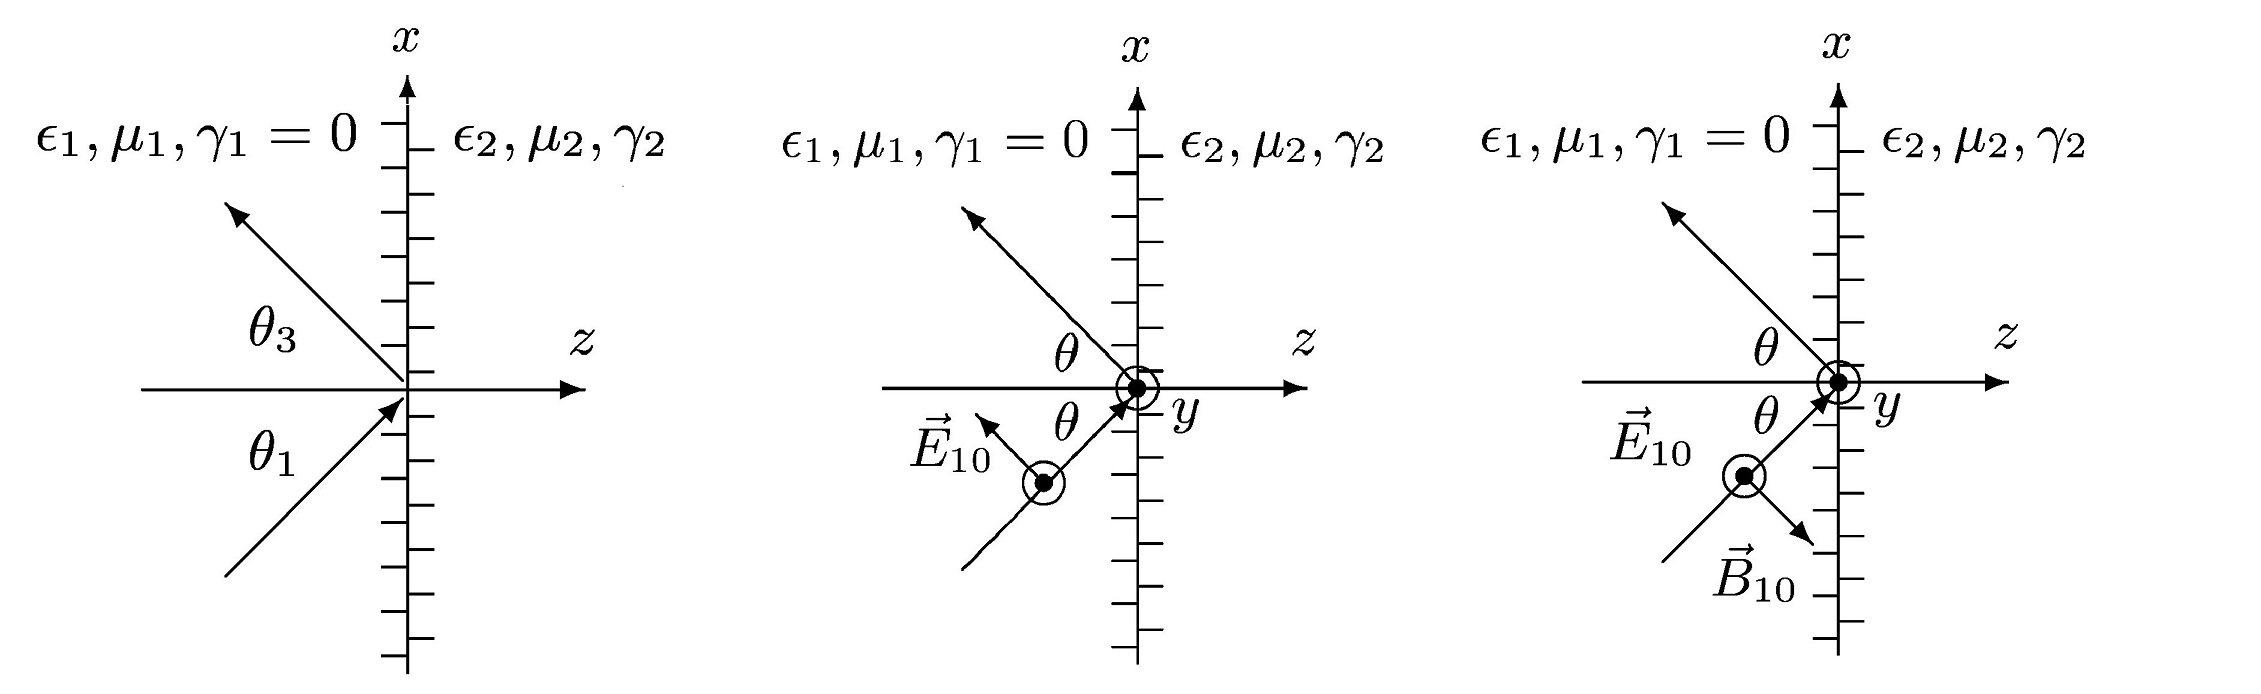
\includegraphics[width=1.2\linewidth]{note_Wave_Reflect.jpg}
      \caption{电磁波反射示意\label{fig:wave_reflect}}
    \end{figure}
\begin{enumerate}
    \item 基本方程
    \begin{align}
        &\uvec e_n\times(\vec E_1 + \vec E_3 - \vec E_2) = 0 \\
        &\uvec e_n\times(\vec H_1 + \vec H_3 - \vec H_2) = \vec \alpha \\
        &\uvec e_n\cdot(\vec D_1 + \vec D_3 - \vec D_2) = \sigma \\
        &\uvec e_n\cdot(\vec B_1 + \vec B_3 - \vec B_2) = 0
    \end{align}
    \item 波矢量的变化: 
    \begin{align}
        &k_{1x} = k_{2x} = k_{3x}, k_{1y} = k_{2y} = k_{3y}\\
        &k^2 = \omega^2\mu\varepsilon + \mi\omega\mu\gamma
    \end{align}
     \begin{itemize}
         \item 反射波 $\theta_3 = \theta_1$ 反射定律.
         \item 透射波\footnote{要求 $k_{2z\mathrm R}$ 正的实数解} 
         \begin{align}
             k_{2x} &= \sqrt{\mu_1\varepsilon_1}\omega\sin\theta_1, &k_{2y} &= 0
         \end{align}
         \begin{align}
             k_{2z\mathrm R} &= \frac1{\sqrt 2}\sqrt{k_{z0}^2 + \sqrt{k_{z0}^4 + \mu_2^2\gamma_2^2\omega^2}} \\
             k_{2z\mathrm I} &= \frac{\omega\mu_2\gamma_2}{\sqrt2\sqrt{k_{z0}^2 + \sqrt{k_{z0}^4 + \mu_2^2\gamma_2^2\omega^2}}}
         \end{align}
         其中 $k_{z0}^2 =(\mu_2\varepsilon_2 - \mu_1\varepsilon_1\sin^2\theta_1)\omega^2$
         \begin{itemize}
             \item 标准折射情形 $\gamma_2 = 0, \sin\theta_1\le\sqrt{\mu_2\varepsilon_2/\mu_1\varepsilon_1} = n_2/n_1$ 
             \begin{align}
                 k_{2z\mathrm I} &= 0,& k_{2z\mathrm R} &= \sqrt{k_{z0}^2}, &n_2\sin\theta_2 = n_1\sin\theta_1
             \end{align}
             \item 全反射情形 $\gamma_2 \to 0, \sin\theta_1\le\sqrt{\mu_2\varepsilon_2/\mu_1\varepsilon_1} > n_2/n_1$ 
             \begin{align}
                 k_{2z\mathrm R} &= 0,& k_{2z\mathrm I} &= \sqrt{-k_{z0}^2}
             \end{align}
             透射波
             \begin{equation}
                 \vec X_2 = \vec X_{20}\e^{-\omega z\sqrt{\mu_1\varepsilon_1\sin\theta_1 - \mu_2\varepsilon_2}}\e^{\mi(\omega x\sqrt{\mu_1\varepsilon_1}\sin\theta_1 - \omega t)}
             \end{equation}
         \end{itemize}
     \end{itemize}
    \item 复振幅的变化:
    \begin{itemize}
        \item 电场平行于入射面 
        \begin{align}
            \vec E_{20\parallel} &= \frac{2\cos\theta_1}{\frac{k_{2z}}{k_2}+\frac{\mu_1k_2\cos\theta_1}{\mu_2k_1}}E_{10\parallel}\left(\frac{k_{2z}}{k_2}\uvec e_1 - \frac{k_{2x}}{k_2}\uvec e_3\right) \\
            &\stackrel{*}{=} \frac{2\cos\theta_1\sin\theta_2}{\sin(\theta_1+\theta_2)\cos(\theta_2-\theta_2)}E_{10\parallel}\uvec e_{2\parallel} \label{equ_frepara2}
         \end{align}
         \begin{align}
            \vec E_{30\parallel} &= \frac{-\frac{k_{2z}}{k_2} + \frac{\mu_1k_2}{\mu_2k_1}\cos\theta_1}{\frac{k_{2z}}{k_2} + \frac{\mu_1k_2}{\mu_2k_1}\cos\theta_1}E_{10\parallel}\left(\frac{k_{3z}}{k_3}\uvec e_1 - \frac{k_{3x}}{k_3}\uvec e_3\right) \\
            &\stackrel{*}{=} \frac{\tan(\theta_1-\theta_2)}{\tan(\theta_1+\theta_2)}E_{10\parallel}\uvec e_{3\parallel} \label{equ_frepara3}
        \end{align}
        其中 $* : \gamma_2 = 0, \mu_1= \mu_2$
        \item 电场垂直入射面
        \begin{align}
            \vec E_{20\perp} &= \frac{2}{1+\frac{\mu_1k_{2z}}{\mu_2k_1\cos\theta_1}}E_{10\perp}\uvec e_2 \\
            &\stackrel{*}{=} \frac{\sin(\theta_2 - \theta_1)}{\sin(\theta_2 + \theta_1)}E_{10\perp}\uvec e_2 \label{equ_freperp2}
         \end{align}
         \begin{align}
            \vec E_{30\perp} &= \frac{1-\frac{\mu_1k_{2z}}{\mu_2k_1\cos\theta_1}}{1+\frac{\mu_1k_{2z}}{\mu_2k_1\cos\theta_1}}E_{10\perp}\uvec e_2 \\
            &\stackrel{*}{=} \frac{2\sin\theta_2\cos\theta_1}{\sin(\theta_2 + \theta_1)}E_{10\perp}\uvec e_2 \label{equ_freperp3}
        \end{align}
        \begin{itemize}
            \item 半波损失: 考察反射波和透射波的方向
            \begin{itemize}
                \item $\vec E_{20}$ 无半波损失
                \item $\vec E_{30}$ 在 $n_1>n_2, \theta_1\to 0$ 时无半波损失, 其他时候有半波损失
            \end{itemize}
            \item Fresnel 公式: 式 (\ref{equ_frepara2}), (\ref{equ_frepara3}), (\ref{equ_freperp2}), (\ref{equ_freperp3})
            \item Brewster 定律: 式 (\ref{equ_frepara3}) 中 $\theta_1 + \theta_2 = \pi/2$ 时, $E_{\parallel}$ 不反射, 此时的 $\theta$ 为 Brewster 角
            \item 能流密度
            \begin{align}
                \langle\vec S_{3\parallel}\rangle &=  \frac{\vec k_3}{2\mu_1\omega}\Vert E_{30\parallel}\Vert^2 &
                \langle\vec S_{3\perp}\rangle &= \frac{\vec k_3}{2\mu_1\omega}\Vert E_{30\perp}\Vert^2
            \end{align}
            \begin{align}
                \langle\vec S_{2\parallel}\rangle &= \frac{\Vert E_{2\parallel}\Vert^2\vec k_{2\mathrm R} - \Re[(\vec k_2\cdot\vec E_{2\parallel}^*)(\vec E_{2\parallel} + \vec E_{2\perp})]}{2\mu_2\omega} \\
                \langle\vec S_{2\parallel}\rangle &= \frac{\vec k_{2\mathrm R}}{2\mu_2\omega}\Vert\vec E_{2\perp}\Vert^2
            \end{align}
            值得注意的是, 可能有传导电流时, $\rangle\vec S_2 \langle$ 形式特别, 不能仅看复振幅部分 (无下标 $0$), 同时平行能流与电场垂直分量有关
            \item 透射率 $D$ 与反射率 $R$
            \begin{align}
                D_\perp &= \left.\frac{\langle S_{2\perp z}\rangle}{\langle S_{1\perp z}\rangle}\right|_{z=0} = \frac{\mu_1k_{2z\mathrm R}}{\mu_2k_1\cos\theta_1}\left\Vert\frac{2}{1+\frac{\mu_1k_{2z}}{\mu_2k_1\cos\theta_1}}\right\Vert^2 \\
                R_\perp &= -\left.\frac{\langle S_{3\perp z}\rangle}{\langle S_{1\perp z}\rangle}\right|_{z=0} = \left\Vert\frac{1-\frac{\mu_1k_{2z}}{\mu_2k_1\cos\theta_1}}{1+\frac{\mu_1k_{2z}}{\mu_2k_1\cos\theta_1}}\right\Vert^2 = 1-D_\perp \\
                D_\parallel &= \frac{4\mu_1\cos\theta_1\Re[k_2k_{2z}^*/k_2^*]}{\mu_2k_1\left\Vert\frac{k_{2z}}{k_2} + \frac{k_2\mu_1}{k_1\mu_2}\cos\theta_1\right\Vert^2} \\
                R_\parallel &= \left\Vert\frac{\frac{k_{2z}}{k_2} - \frac{k_2\mu_1}{k_1\mu_2}\cos\theta_1}{\frac{k_{2z}}{k_2} + \frac{k_2\mu_1}{k_1\mu_2}\cos\theta_1}\right\Vert^2 = 1-D_\parallel
            \end{align}
        \end{itemize}
    \end{itemize}
\end{enumerate}
% subsection reflect_and_refraction (end)
\subsection{谐振腔与波导} % (fold)
\label{sub:resonant_cavity_and_wave_guide}
\begin{enumerate}
    \item 谐振腔, 边界理想导体的条件
    \begin{equation}
        \vec E_{\parallel} = 0, \qquad \frac{\partial E_n}{\partial \uvec n} = 0
    \end{equation}
    \begin{itemize}
        \item 以矩形谐振腔为例, 由边界条件分离变量得到振动模式
        \begin{align}
            E_x &= A_x\cos k_x x \sin k_y y \sin k_z z \\
            E_y &= A_y\sin k_x x \cos k_y y \sin k_z z \\
            E_z &= A_z\sin k_x x \sin k_y y \cos k_z z
        \end{align} 
        其中 $k_i = n_i\pi/L_i$, 至少应有 $2$ 个不为 $0$. 再由 $\nabla\cdot \vec E = 0$ 得到
        \begin{equation}
            k_i A_i = 0
        \end{equation}
    \end{itemize}
    \item 波导: $x-y$ 谐振腔, $z$ 向传播. 
    \begin{equation}
        \vec X = \left[\vec X_z(x,y) + \vec X_t(x,y)\right]\e^{\mi k_z z}
    \end{equation}
    满足方程 $\nabla_{xy}\cdot\vec X_t + \mi k_z X_z = 0$, 以及边界条件 $\uvec n\times\vec E = 0$, (可以具有管壁上的面电流 $\vec i = \uvec n\times\vec H$ 和电荷 $\sigma = \uvec n\cdot\vec D$). 分解不同的振动模式
    \begin{itemize}
        \item TEM 波: $E_z = B_z = 0$, 退化为二维静电问题
        \item TE 波: $E_z = 0$, 导出 $(\nabla^2_{xy}+\mu\varepsilon\omega^2-k_z^2)B_z = 0$, 截止频率 $\omega_c\ge\left(k_x^2+k_y^2\right)/\mu\varepsilon$
        \item TM 波: $B_z = 0$
    \end{itemize}
    特别的对于矩形波导, 可以解得振动模式 $(m,n)$
    \begin{align}
        E_x &= A_1\cos\left(m\pi\frac xa\right)\sin\left(n\pi\frac yb\right)\e^{\mi k_z z} \\
        E_y &= A_2\sin\left(m\pi\frac xa\right)\cos\left(n\pi\frac yb\right)\e^{\mi k_z z} \\
        E_z &= A_3\sin\left(m\pi\frac xa\right)\sin\left(n\pi\frac yb\right)\e^{\mi k_z z}
    \end{align}
    限制条件 $k_xA_1 + k_y A_2 - \mi k_z A_3 = 0$
\end{enumerate}
% subsection resonant_cavity_and_wave_guide (end)
\subsection{电磁波的几何光学极限} % (fold)
\label{sub:limit_geometry}
    对于非均匀介质, 在什么情况下能够讨论电磁波的轨迹? 
    讨论 $\mu = \mbox{const.}$ 的情形, 则
    \begin{equation}
        \nabla^2 E - \frac 1{v^2}\frac{\partial^2\vec E}{\partial t^2} 
        = -\nabla\left[(\nabla\ln\varepsilon)\cdot\vec E\right]
    \end{equation}
    其中介质中光速 $v = c/n(\vec r)$, 并且假定定态电磁波的解的形式
    \begin{equation}
        \vec X(\vec r, t) = \vec X_0(\vec r) \e^{\mi\Phi(\vec r) - \mi\omega t}
    \end{equation}
    其中 $\vec X_0, \Phi$ 均为实函数, 满足电磁学方程, 得到
    \begin{align}
        &\nabla\cdot\vec E = -(\nabla\ln\varepsilon)\cdot\vec E
        &\Rightarrow& \nabla\cdot\vec E_0 = -\left(\nabla\ln\varepsilon\right)\cdot\vec E_0, \quad (\nabla\Phi)\cdot\vec E_0 = 0 \\
        &\nabla^2 \vec E - \frac 1{v^2}\frac{\partial^2\vec E}{\partial t^2} 
        = -\nabla\left[(\nabla\ln\varepsilon)\cdot\vec E\right]
        &\Rightarrow& \begin{array}{l}
            \nabla^2\vec E_0 - \vec E_0\left(\nabla\Phi\right)^2+ \vec E_0\frac{\omega^2}{v^2} = \nabla(\nabla\cdot\vec E) \\
            \nabla\cdot(\vec E_0^2\nabla\Phi) = 0
        \end{array}
    \end{align}
    几何光学近似要求 $\vec E_0$ 随空间变化缓慢, 于是近似的 $(\nabla\Phi)^2 = \omega^2/v^2$, $\vec E_0\cdot\nabla\epsilon = 0$.\\
    电磁波轨迹 $\vec r(s)$ 定义为等相面的法线的轨迹, 也即
    \begin{equation}
        \nabla\Phi = \frac\omega v\frac{\dif\vec r}{\dif s}
    \end{equation}
    仍然有 $\vec E, \vec B, \dif\vec r$ 的右手关系 (近似), 定义光程泛函
    \begin{equation}
        \Phi(\vec r_1, \vec r_2)\equiv\int_{\vec r_1}^{\vec r_2}\dif r n(\vec r)
    \end{equation}
    代入上述关系可以证明费马原理
% subsection limit_geometry (end)
\subsection{衍射} % (fold)
\label{sub:diffraction}
定义 $\vec R  = \vec r' - \vec r$, $t^* = t - R/c$ (记 $t^*$ 时求偏导表示保持 $t^*$ 不变的偏导), 在满足波动方程的条件下, 具有恒等式
\begin{align*}
    u(\vec r, t) &= \int\dif \tau'\delta(\vec r' - \vec r) u(\vec r', t-R/c) \\
    &= -\frac 1{4\pi}\int\dif \tau'\left(\nabla'^2\frac 1R\right) u(\vec r', t-R/c)\\
    &= \frac 1{4\pi}\int\dif \vec S' \cdot \left[\frac 1R\nabla'u(\vec r',t^*) + \frac{\vec R}{R^3}u(\vec r',t^*) + \frac{\vec R}{cR^2}\frac{\partial}{\partial t^*}u(\vec r,t^*)\right]
\end{align*}
对于小孔, 代入 Kirchhoff 假设:
\begin{itemize}
    \item 除了孔 $\Delta S$, $u$, $\nabla u$ 在界面 $S$ 上处处为零
    \item 孔内与无障碍相同:
    \begin{equation}
        u(\vec r, t) = \begin{cases}
            0 & \vec r\in S/\Delta S \\
            A\e^{\mi\omega(t-z/c)} &\vec r\in\Delta S
        \end{cases}
    \end{equation}
\end{itemize}
同时假定 $\dif\vec S' = -\dif S'\uvec e_z$ (取负号是由于正向是考察空间指向外侧), 于是
\begin{equation}
    u(\vec r,t) = \frac A{4\pi}\int_{\Delta S}\dif S\left[\frac{\mi\omega}{cR}(1+\cos\theta) + \frac{\cos\theta}{R^2}\right]\e^{-\mi\omega R/c}
\end{equation}
\begin{itemize}
    \item 当孔距屏较远时, 主要第一项贡献: Fraunhofer 衍射
    \item 当孔距屏较近时, 主要第二项贡献: Fresnel 衍射
\end{itemize}
% subsection diffraction (end)
% section EMW (end)

\section{电磁辐射} % (fold)
\label{sec:radiation}
需要用到的前文公式抄录如下
\begin{itemize}
    \item (真空中的) d'Alembert 方程, 与 Maxwell 方程组等价
    \begin{align}\label{equ:dalembert}
        &\left(\nabla^2- \frac 1{c^2}\frac{\partial^2}{\partial t^2}\right)\vec A - \nabla\left(\nabla\cdot\vec A + \frac 1{c^2}\frac{\partial \varphi}{\partial t}\right) = -\mu_0\vec j \\
        \nabla^2\varphi - \frac{\partial}{\partial t}\nabla\cdot\vec A = 
        &\left(\nabla^2- \frac 1{c^2}\frac{\partial^2}{\partial t^2}\right)\varphi + \frac{\partial}{\partial t}\left(\nabla\cdot\vec A + \frac 1{c^2}\frac{\partial \varphi}{\partial t}\right) = -\frac{\rho}{\varepsilon_0}
    \end{align}
    \item 规范变换
    \begin{align}\label{equ:gauge_trans}
     \vec A &\rightarrow \vec A + \nabla\chi 
     &\varphi &\rightarrow \varphi - \frac{\partial\chi}{\partial t}
    \end{align}
    \item Coulomb 规范
    \begin{equation}
        \nabla\cdot\vec A = 0\Longrightarrow 
        \nabla\vec A - \frac 1{c^2}\frac{\partial^2\vec A}{\partial t^2} = -\mu_0\vec j + \frac 1{c^2}\frac{\partial}{\partial t}\nabla\varphi \equiv -\mu_0\vec j^* \quad
        \nabla^2\varphi = -\frac{\rho}{\varepsilon_0}
    \end{equation}
    \item Lorenz 规范
    \begin{equation}\label{equ:lorenz_gauge}
        \nabla\cdot\vec A + \frac 1{c^2}\frac{\partial \varphi}{\partial t} = 0\Longrightarrow
        \nabla^2\vec A - \frac 1{c^2}\frac{\partial^2\vec A}{\partial t^2} = -\mu_0\vec j \quad
        \nabla^2\varphi - \frac 1{c^2}\frac{\partial^2\varphi}{\partial t^2} = -\frac{\rho}{\varepsilon_0}
    \end{equation}
\end{itemize}
\subsection{推迟势} % (fold)
\label{sub:retarded_potential}
推迟势, 从 Lorenz 规范 (式\ref{equ:lorenz_gauge}) 中的电势方程出发, 定义格林函数 $U$
\begin{equation}
    \nabla^2 U(\vec r,\vec r', t) - \frac 1{c^2}\frac{\partial^2}{\partial t^2} U(\vec r,\vec r', t) = -\frac{\rho(\vec r',t)}{\varepsilon_0}\delta(\vec r - \vec r');\quad 
    \varphi(\vec r, t) = \int\dif \tau' U(\vec r, \vec r', t)
\end{equation}
由对称性 $U(\vec r,\vec r', t) = U(R,\vec r', t)$, 
其中 $R = |\vec R| = |\vec r - \vec r'|$, 代入得到
\begin{equation}
    \nabla^2 U = \frac 1R\frac{\partial^2(RU)}{\partial R^2};\quad 
    \frac{\partial^2 (RU)}{\partial R^2} - \frac 1{c^2}\frac{\partial^2(RU)}{\partial t^2} = -\frac 1{\varepsilon_0}\delta(\vec R)\rho(\vec r',t)R = 0
\end{equation}
由 $RU$ 的波动方程形式, 可知特解 $U_1 = f(t-R/c,\vec r')/R$ (推迟解), $U_2 = g(t+R/c,\vec r')/R$ (超前解), 代入方程解得 $f = \rho(\vec r',t-R/c)/4\pi\varepsilon_0$, $g = \rho(\vec r', t+R/c)/4\pi\epsilon$, 由两者的对称性得到
\begin{align}
    \varphi(\vec r, t) &= \int\dif \tau'\frac{\rho(\vec r',t-R/c)}{4\pi\varepsilon_0 R} 
    &\vec A(\vec r, t) &= \int\dif \tau'\frac{\mu_0\vec j(\vec r', t-R/c)}{4\pi R}
    &\mbox{Lorenz 规范} \label{equ:retarded_potential_lg}\\
    \varphi(\vec r, t) &= \int\dif \tau'\frac{\rho(\vec r',t)}{4\pi\varepsilon_0 R} 
    &\vec A(\vec r, t) &= \int\dif \tau'\frac{\mu_0\vec j^*(\vec r', t-R/c)}{4\pi R}
    &\mbox{Coulomb 规范}
\end{align}
Coulomb 规范中 $\vec j^*\equiv \vec j - \epsilon_0\nabla(\partial\varphi/\partial t)$.

光子质量假设 $m$, 于是方程变为
\begin{equation}
    \left(\nabla^2 - \frac 1{c^2}\frac{\partial^2}{\partial t^2} - \frac{m^2c^2}{\hbar^2}\right)\tilde\varphi(\vec r, t) = -\frac{\rho(\vec r,t)}{\varepsilon_0}
\end{equation}
对于稳恒场得到的格林函数解 $\tilde U = U\e^{-mcR/\hbar}$. 
% subsection retarded_potential (end)
\subsection{光子质量假设与超导} % (fold)
\label{sub:mass_of_photon}
如果在某种介质中具有电荷, 电流形式
\begin{equation}
    \vec j = -\frac{m^2c^2}{\mu_0\hbar^2}{\vec A}, \qquad
    \rho = -\frac{m^2\varepsilon_0 c^2}{\hbar^2}\varphi
\end{equation}
则相当于在 d'Alembert 方程中加入了光子质量 (式\ref{equ:dalembert}), 并且由电荷守恒 $\nabla\cdot\vec j + \partial\rho/\partial t = 0$ 导出 Lorenz 规范
\begin{align}
    &\left(\nabla^2- \frac 1{c^2}\frac{\partial^2}{\partial t^2} - \frac{m^2c^2}{\hbar^2}\right)\vec A = -\mu_0\vec j \\
    &\left(\nabla^2- \frac 1{c^2}\frac{\partial^2}{\partial t^2} - \frac{m^2c^2}{\hbar^2}\right)\varphi = -\frac{\rho}{\varepsilon_0}
\end{align}
此时规范对称性破缺. 此时由势的定义 $\nabla\times\vec A = \vec B$, $\nabla\varphi + \partial\vec A/\partial t = -\vec E$ 分布导出 London 第一, 第二方程. 而电流不能随时间指数增长保证了电导率 $\gamma = \infty$; 并导出磁场和电流随穿透距离指数衰减 (Meissner 效应).

反之, 若发生超导, 则 London 方程成立, 搭配 Lorenz 协变性并且选择合适的规范可以得等效光子质量. 

由 London 方程也可以得到不影响规范对称性的形式
\begin{equation}
    \mu_0\vec j = \frac{m^2c^2}{\hbar^2}\left(\vec A + \nabla\chi\right) \qquad
    \frac{\rho}{\varepsilon_0} = \frac{m^2c^2}{\hbar^2}\left(\varphi - \frac{\partial \chi}{\partial t}\right)
\end{equation}
% subsection mass_of_photon (end)
\subsection{辐射电磁场} % (fold)
\label{sub:radation_field}
仅保留 $\vec B$, $\vec E$ 中不低于 $1/R$ 的项, 因而只需要对 $t^*$ 求导即可
\begin{align}
    \vec B_r &\equiv \left.\left(\nabla\times\vec A\right)\right|_{1/r} 
    = \int\dif \tau'\frac{\mu_0}{4\pi cR}\frac{\partial\vec j^*}{\partial t}\times\uvec n \\
    \vec E_r &\equiv \left.\left(-\nabla\varphi - \frac{\partial\vec A}{\partial t}\right)\right|_{1/r} 
    = \int\dif \tau'\frac{\mu_0}{4\pi R}\left[\left(\frac{\partial\vec j^*}{\partial t}\cdot\uvec n\right)\uvec n - \frac{\partial\vec j^*}{\partial t}\right]
\end{align}
其中 $t^*\equiv t-R/c$, $\uvec n \equiv \vec R/R$, $\vec j^*\equiv \vec j(\vec r',t^*)$. 辐射场满足:
\begin{itemize}
     \item 右手关系 $\uvec n\times\vec E_r = c\vec B_r$, $c\vec B_r \times\uvec n = \vec E_r$
     \item 能量密度 $W_e = \varepsilon_0 E^2/2 = W_m = B^2/2\mu_0$
     \item 能流密度 $\vec S \equiv \vec E\times\vec H = (W_e + W_m)c\uvec n$
\end{itemize} 
% subsection radation_field (end)
\subsection{辐射磁场的多极展开} % (fold)
\label{sub:radiation_field_multipole}
磁矢量势的多极展开 (与式(\ref{equ:multipole_for_A}) 的差异是这里仅保留 $1/r$ 项, 因而只需要对 $t^*$ 展开)
\begin{equation}
    \vec A_r (\vec r,t) = \frac{\mu_0}{4\pi r}\sum_{k=0}^{\infty}
    \frac 1{k!}\frac 1{c^k R^k} \prod_{p=1}^k R_{i_p}\frac{\partial^k}{\partial t^k} 
    \vec J_{i_1, i_2, \cdots, i_k}\left(t - \frac rc\right)
\end{equation}
其中磁多级矩的定义与式(\ref{equ:mag_multipole}) 相同
\begin{equation}
    \vec J_{i_1, i_2, \cdots, i_k}\equiv\int\dif \tau'\vec j(\vec r', t)\prod_{p=1}^k x'_{i_p}
\end{equation}
于是磁场
\begin{equation}
    \vec B_r = \sum_{k=0}^\infty \vec B_k \equiv \sum_{k=0}^\infty \left[
    \frac{\mu_0}{4\pi r}\frac 1{k!}\frac 1{c^k R^k} \prod_{p=1}^k R_{i_p}\frac{\partial^{k+1}}{\partial t^{k+1}} \vec J_{i_1, i_2, \cdots, i_k}\left(t - \frac rc\right)\times\uvec n\right]
\end{equation}
讨论相邻两项
\begin{equation}
    \left|\frac{B_{k+1}}{B_k}\right| \sim \left|\frac{x'}{c}\frac{\partial}{\partial t}\right|\sim\frac{l'\nu}{c} = \frac{l'}{\lambda}
\end{equation}
其中 $l'$ 表示电荷体系的线度, $\lambda$ 表示对应的辐射波长. 因此仅对于长波辐射 (如无线电等) 这样的做法是有效的.

零级仅与电偶极 $\vec p \equiv \int\dif \tau'\vec r'\rho$ 有关, 称电偶极辐射
\begin{equation}
    \vec B_0 = \frac{\mu_0}{4\pi cr}\ddot{\vec p}(t-r/c)\times\uvec n
\end{equation}

一级则是磁偶极辐射和电四级辐射
\begin{equation}
    \vec B_1 = \frac{\mu_1}{4\pi c^2 r}\left[\frac 16 n_i\dddot{\mathscr D_{ij}}(t-r/c) \uvec e_j + \ddot{\vec m}(t-r/c)\times\uvec n\right]\times\uvec n
\end{equation}
其中电四极矩与式(\ref{equ:elctro_quadrupole}) 相同, 磁偶极矩 $\vec m \equiv 2^{-1}\int\dif \tau'\vec r'\times\vec j$ 与式(\ref{equ:mag_dipole}) 相同
% subsection radiation_field_multipole (end)
% section radiation (end)

\section{狭义相对论} % (fold)
%暂且按照王青和郭硕鸿的方法, 有空了按照逆变和协变的格式重新写一遍
\label{sec:special_relativity}
\subsection{Lorentz 变换} % (fold)
\label{sub:lorentz_trans}
变换矩阵 $aa_{\mu\nu}a_{\mu\lambda} = \delta_{\nu\lambda}$
\begin{equation}
    a = \begin{pmatrix}
        \gamma          & 0 & 0 &\mi\beta\gamma \\
        0 & 1 & 0 & 0 \\
        0 & 0 & 1 & 0 \\
        -\mi\beta\gamma & 0 & 0 &\gamma         \\
    \end{pmatrix}
\end{equation}
对应坐标定义 $X = (x,y,z,\mi ct)^T$. 在外微分记号的意义下, 四维体积元 $\dif t\dif \tau = \dif^4 X /\mi c$ 是标量
\begin{itemize}
    \item 变换的线性由空间均匀得出: 形成 Lorentz 群
    \item 更一般的 $x'_\mu = a_{\mu\nu}x_\nu + b_\mu$, 形成 Poincar\'e 群, 导致 Minkovski 时空
    \item 最一般的, 保证惯性定律 $x = x_0 + v(t-t_0)$ 成立的, 华罗庚惯性运动群
\end{itemize}
物理量应均由协变张量表达, 从而满足相对论
% subsection lorentz_trans (end)
\subsection{最小作用量原理表达的狭义相对论} % (fold)
\label{sub:min_action}
\subsubsection{单粒子作用量} % (fold)
\label{ssub:single_partical}
孤立单粒子的 Lagrange 量, 其中 $\dif s =\sqrt{-\dif X_\mu\dif X_\mu} = \sqrt{c^2(\dif t)^2 - (\dif x)^2}$ 
\begin{equation}
    S = -m_0c\int\dif s = -m_0c^2\int\dif t\sqrt{1-\frac{\dot x^2}{c^2}} = \int\dif tL
\end{equation}
导出共轭动量和哈密顿量
\begin{equation}
    p_i = \frac{\partial L}{\partial \dot x_i} = \frac{m_0\dot x_i}{\sqrt{1 - v^2/c^2}} \qquad 
    H = p_i v_i - L = \frac{m_0 c^2}{\sqrt{1-v^2/c^2}}
\end{equation}
四维动量与之一致
\begin{equation}
    P_\mu = m_0\frac{\dif X_\mu}{\dif \tau} = (p_1, p_2, p_3, \mi H/c)
\end{equation}
定义四维势 $A = (A_x, A_y, A_z, \mi\varphi/c)$, 
% subsubsection single_partical (end)
\subsubsection{单粒子与电磁场耦合} % (fold)
\label{ssub:single_particle_with_EMF}
在上面的式子加入电磁场与粒子的最小耦合项
\begin{equation}
    S = -m_0c\int\dif s + e\int\dif X_\mu A_\mu 
    = \int\dif t\left(-m_0 c^2\sqrt{1-\frac{v^2}{c^2}} + e\vec A\cdot\vec v - e\varphi\right)
\end{equation}
值得注意的是, 这样的取法直接满足了规范变换
\begin{equation}
    A_\mu\to A_\mu' = A_\mu + \partial_\mu \chi
\end{equation}
据此共轭动量与哈密顿量以及 Lorentz 力公式
\begin{align}
    &\vec p = \frac{m_0\vec v}{\sqrt{1-v^2/c^2}} + e\vec A\qquad
    H = \frac{m_0 c^2}{\sqrt{1-v^2/c^2}} + e\varphi \\
    &\frac{\dif}{\dif t}\frac{m_0\vec v}{\sqrt{1-v^2/c^2}} 
    = e(-\frac{\partial\vec A}{\partial t} - \nabla\varphi) + e\vec v\times(\nabla\times\vec A) = e\vec E + e\vec v\times\vec B
\end{align}
推广到连续的情形, 引入四维电流密度 $J = (\vec j, \mi c\rho)$, 最小耦合项变为
\begin{equation}
    \int\dif t\dif \tau A_\mu J_\mu = \int\dif t\dif \tau (\vec A\cdot\vec j - \varphi\rho)
\end{equation}
此时引入规范对称性, 要求变换不影响作用量, 则得出电荷守恒 (规范对称性的 Noether 流是电流)
\begin{align}
    &0 = \int\dif t\dif \tau J_\mu\partial_\mu\chi = -\int\dif t\dif\tau(\partial_\mu j_\mu)\chi \\
    \Longleftrightarrow\quad& \partial_\mu J_\mu = 0 \quad\Leftrightarrow\quad \frac{\partial\rho}{\partial t} + \nabla\cdot\vec j = 0
\end{align} 
% subsubsection single_particle_with_EMF (end)
\subsubsection{完整的电动力学表述} % (fold)
\label{ssub:all_elemag_in_action}
引入电磁场张量 $F_{\mu\nu} = \partial_\mu A_\nu - \partial_\nu A_\mu$, 并据此有电磁场的 Lorentz 变换
\begin{equation}
    F = \begin{pmatrix}
        0         &  B_z       & -B_y       & -\mi E_x/c \\
       -B_z       &  0         &  B_x       & -\mi E_y/c \\
        B_y       & -B_x       &  0         & -\mi E_z/c \\
       \mi E_x/c & \mi E_y/c & \mi E_z/c & 0          
    \end{pmatrix}
\end{equation}
具有四矢量形式的力密度, 以及对于点电荷的四维力形式
\begin{align}
    &f_\mu = F_{\mu\nu}J_\nu,\qquad f = (\rho\vec E + \vec j\times\vec B, \mi\vec j\cdot\vec E/c) \\
    &K_\mu = m_0\frac{\dif u_\mu}{\dif\tau} = eF_{\mu\nu}u_\nu
\end{align}
在作用量中加入满足规范不变性的项, 其中第二项仅与边界有关, 以下咱不讨论
\begin{equation}\label{equ:field_in_action}
    F_{\mu\nu}F_{\mu\nu} = 2\left(B^2 - \frac{E^2}{c^2}\right), \qquad
    \epsilon_{\mu\nu\sigma\rho} F_{\mu\nu} F_{\sigma\rho} 
    = -\frac{8\mi}c \vec E\cdot\vec B 
    = 4\epsilon_{\mu\nu\sigma\rho}\partial_\mu(A_\nu\partial_\sigma A\rho)
\end{equation}
相应的电磁场相关作用量变为
\begin{equation}
    S = \int\dif t\dif\tau \left(-\frac 1{4\mu_0}F_{\mu\nu}F_{\mu\nu} + J_\mu A_\mu\right)
\end{equation}
由最小作用量原理得出 (的结构满足流守恒方程 $\partial_\mu J_\mu = -\mu_0^{-1}\partial_\mu\partial_\nu F_{\mu\nu} = 0$)
\begin{equation}
    \partial_\mu F_{\mu\nu} = -\mu_0 J_\nu \qquad\Longleftrightarrow\qquad
    \nabla\times\vec B = \mu_0\vec j + \frac 1{c^2}\frac{\partial\vec E}{\partial t},
    \quad \nabla\cdot\vec E = \frac{\rho}{\varepsilon_0}
\end{equation}
Maxwell 方程组的另外两个式子由 $F_{\mu\nu} = \partial_\mu A_\nu - \partial_\nu A_\mu$ 的结构给出
\begin{equation}
    \partial_\mu F_{\nu\lambda} + \partial_\nu F_{\lambda\mu} + \partial_\lambda F_{\mu\nu} = 0 \qquad \Longleftrightarrow \qquad 
    \nabla\cdot\vec B = 0, \quad 
    \nabla\times\vec E = -\frac{\partial\vec B}{\partial t}
\end{equation}
% subsubsection all_elemag_in_action (end)
% subsection min_action (end)
\subsection{电磁物理量的张量表达} % (fold)
\label{sub:tensor_express_of_EMF}
\subsubsection{介质} % (fold)
\label{ssub:medium_under_relativity}
包含介质的 Maxwell 方程
\begin{equation}
    \nabla\cdot\vec D = \nabla(\varepsilon_0\vec E + \vec P) = \rho_f \qquad
    \nabla\times\vec H = \vec j_c + \frac{\partial}{\partial t}(\varepsilon_0\vec E + \vec P)
\end{equation}
得知 $\vec P/\varepsilon_0$ 与 $\vec E$, $-\mu_0\vec M$ 与 $\vec B$ 应满足相同的变换关系, 定义极化张量
\begin{equation}
    M \equiv \begin{pmatrix}
        0        & -M_z      &  M_y      & -\mi cP_x \\
        M_z      &  0        & -M_x      & -\mi cP_y \\
       -M_y      &  M_x      &  0        & -\mi cP_z \\
        \mi cP_x &  \mi cP_y &  \mi cP_z &  0
    \end{pmatrix}
\end{equation}
% subsubsection medium_under_relativity (end)
% subsection tensor_express_of_EMF (end)
\subsubsection{动量流密度与能流密度} % (fold)
\label{ssub:dynamic_density}
从力密度 $f_\mu$ 出发
\begin{equation}\label{equ:force_density_and_tensor}
    f_\mu = F_{\mu\nu}J_\nu = -\frac 1{\mu_0}F_{\mu\nu}\partial_\lambda F_{\lambda\nu}
     = -\frac 1{\mu_0}\partial_\nu\left(F_{\mu\sigma}F_{\nu\sigma} - \frac 14\delta_{\mu\nu}F_{\sigma\lambda}F_{\sigma\lambda}\right) \equiv -\partial_\nu T_{\mu\nu}
\end{equation}
$T_{\mu\nu}$ 是无迹对称张量 $T_{\mu\mu} = 0, T_{\mu\nu} =T_{\nu\mu}$, 各分量的意义:
\begin{itemize}
    \item 空间分量是动量流密度, 见式(\ref{equ:momentum_density_flux}) $T_{ij} = \mathcal J_{ij}$
    \item 时间分量是能量密度, 见式(\ref{equ:energy_density_and_flux}) $T_{44} = -w$
    \item 交叉分量同时是动量密度和能流密度, 见式(\ref{equ:momentum_density}) $T_{i4} = T_{4i} = \mi c g_i = \mi S_i/c$
\end{itemize}
而式(\ref{equ:force_density_and_tensor}) 展开即为动量守恒与能量守恒
\begin{equation}
    f_i = -\partial_j\mathcal J_{ij},\qquad
    -\mi c f_4 =\vec f\cdot\vec v = -\nabla\cdot\vec S - \frac{\partial w}{\partial t}
\end{equation}

考虑各向同性的 $T$, 静态三维各向同性时, $T = \mathrm{Diag}(p,p,-w)$, 其中 $p$ 是压强, 从而由无迹得到光子气光压 $p = w/3$; 考虑真空四维各向同性, $T = -E_0 \mathcal I$, 其中 $E_0$ 是真空能, 从无迹原则上是 $0$, 如果存在, 则导致表面压力使宇宙膨胀.
% subsubsection dynamic_density (end)
% section special_relativity (end)

\section{带电粒子和电磁场相互作用} % (fold)
\label{sec:elec_partic_and_field}
本章将 \ref{sec:radiation} 章的内容放到点电荷模型下讨论, 并且推广
\subsection{运动带电粒子的电磁场} % (fold)
\label{sub:EMF_of_a_moving_particle}
推迟势的公式与点电荷模型一同使用, 将 $\rho(\vec r, t) = q\delta(\vec r - \vec r_0(t))$, $\vec j(\vec r, t) = q\vec v_0(t)\delta(\vec r - \vec r_0(t))$ 代入式(\ref{equ:retarded_potential_lg}) 中, 得到 Lie\'enard-Wiechert 势
\begin{equation}\label{equ:lw_potential}
    \varphi(\vec r, t) = \frac{q}{4\pi\varepsilon_0|\vec r - \vec r^*|J} \qquad
    \vec A(\vec r,t) = \frac{\mu_0 q\vec v^*}{4\pi|\vec r - \vec r^*|J}
\end{equation}
其中 $\vec r' = \vec r^*$ 是方程 $\vec r' - \vec r_0(t-|\vec r- \vec r'|/c) = 0$ 的解. 并据此定义 $t^* = t-|\vec r - \vec r^*|/c$, $\vec v^* = \vec v_0(t^*)$. 式中 Jacobian 行列式 $J$
\begin{equation}
    J \equiv \left\Vert\frac{\partial}{\partial\vec r'}\left[\vec r' - \vec r_0\left(t-\frac{|\vec r- \vec r'|}{c}\right)\right] \right\Vert_{\vec r' = \vec r^*} 
    = 1 - \frac{(\vec r - \vec r^*)\cdot\vec v^*}{|\vec r - \vec r^*|c}
\end{equation}

根据势的关系得到电场
\begin{align}
    &\vec E(\vec r, t) = \frac{q}{4\pi\varepsilon_0 S^{*3}}\left(\vec R^* - R^*\frac{\vec v^*}c\right)\left(1-\frac{v^{*2}}{c^2}\right)
    + \frac{\mu_0q}{4\pi S^{*3}}\left[\vec R^*\times\left(\left(\vec R^* - R^*\frac{\vec v^*}c\right)\times\vec a^*\right)\right]
\end{align}
式中 $\vec R^* \equiv \vec r - \vec r^*$, $\vec a^* = \vec a_0(t^*)$, $S^*\equiv R^* J = R^*-\vec R^*\cdot\vec v^*/c$. 其中第一项为非辐射场, 第二项为辐射场. 磁场关系 $\vec B(\vec r, t) = \vec R^*\times \vec E(\vec r,t)/cR^*$

其中非辐射场可以化简为
\begin{align}
    \vec E_0 &= \frac{q\vec R}{4\pi\varepsilon_0 S^3}\left(1-\frac{v^{*2}}{c^2}\right)
     =\begin{cases}
         \frac{q\vec R}{4\pi\varepsilon_0 R^3}\left(1-\frac{v^{*2}}{c^2}\right) & \vec R \parallel \vec v^* \\
         \frac{q\vec R}{4\pi\varepsilon_0 R^3}\left(1-\frac{v^{*2}}{c^2}\right)^{-1/2} & \vec R \perp \vec v^*
     \end{cases}
\end{align}
其中 $R = \vec R^* - R^*\vec v^*/c$, $S^2 = (1-v^{*2}/c^2)R^2 + (\vec R\cdot\vec v^*)^2/c^2$. 磁场 $\vec B_0 = \vec v^* \times \vec E_0/c^2$.
\begin{itemize}
    \item 非辐射电场在速度方向上变小, 垂直速度方向上变大
\end{itemize}

考察辐射场关系, 加速运动粒子会产生辐射. 匀速运动粒子当 $v^*\ge c$ 时, 在特定方向上 $S^* = 0$, 出现 $0/0$ 未定式, 也可能产生 Cerekov 辐射. 辐射场能量
\begin{equation}
    \vec S = \frac 1{\mu_0}\vec E_r \times\vec B_r 
    = \frac{q^2\uvec n^*}{16\pi^2\varepsilon_0c^3R^{*2}}
    \frac{|\uvec n^*\times[(\uvec n^* - \vec v^*/c)\times\vec a^*]|^2}{(1-\vec v^*\cdot\uvec n^*/c)^6}
\end{equation}
据此可以得到辐射角分布以及辐射能量
\begin{align}
    &\frac{\dif I^*}{\dif\Omega^*} = \frac{q^2}{16\pi^2\varepsilon_0 c^3}\frac{|\uvec n^*\times[(\uvec n^* - \vec v^*/c)\times\vec a^*]|^2}{(1-\vec v^*\cdot\uvec n^*/c)^5} \\
    &I^* = \frac{q^2}{6\pi\varepsilon_0 c^3}\frac{a^{*2} - (\vec a^{*}\times\vec v^{*})^2/c^2}{(1-v^{*2}/c^2)^3}
\end{align}
\begin{itemize}
    \item $\vec a^*\parallel\vec v^*$, 设 $\theta^*$ 为 $\vec v^* $ 与 $\uvec n^*$ 的夹角
    \begin{align}
        &\frac{\dif I^*}{\dif\Omega^*} = \frac{q^2 a^{*2}\sin^2\theta^*}{16\pi^2\varepsilon_0 c^3(1-v^*\cos\theta^*/c)^5} \\
        &I^* = \frac{q^2a^{*2}}{6\pi\varepsilon_0 c^3(1-v^{*2}/c^2)^3}
    \end{align}
    辐射最强的方向 $\theta^* \le \pi/2$, 且在 $v\to c$ 时 $\theta^*\to 0$
    \item $\vec a^*\perp\vec v^*$, 以 $\vec v^*$ 为 $z$ 轴, $\vec a^*$ 为 $x$ 轴
    \begin{align}
        &\frac{\dif I^*}{\dif\Omega^*} = \frac{q^2 a^{*2}}{16\pi^2\varepsilon_0 c^3(1-v^*\cos\theta^*/c)^3}\left[1-
        \frac{(1-v^{*2}/c^2)\sin^2\theta^*\cos^2\phi^*}{(1-v^*\cos\theta^*/c)^2}\right] \\
        &I^* = \frac{q^2a^{*2}}{6\pi\varepsilon_0 c^3(1-v^{*2}/c^2)^2}
    \end{align}
    辐射分布非轴对称, $\phi^* = 0,\pi$ 最弱, $\phi^* = \pi/2$ 最强. 告诉运动时 $\theta^* = 0$ 最强
\end{itemize}
\subsubsection{辐射频谱分析} % (fold)
\label{ssub:spectral_analysis}
\begin{align}
    \vec E_\omega(\vec r) &= \frac1{2\pi}\int_{-\infty}^{\infty}\dif t\vec E_r(\vec r, t)\e^{\mi\omega t} \\
    &= \frac 1{2\pi}\int_{-\infty}^\infty\dif t^*\e^{\mi\omega t^*} \frac{q\e^{\mi\omega R^*/c}}{4\pi\varepsilon_0 c^2 R^*}\frac{\uvec n^*\times \left[(\uvec n^* - \vec v^*/c)\times\vec a^*\right]}{(1-\uvec n^*\cdot\vec v^*/c)^2} \\
    &=\begin{cases}
        0 & \omega\to\infty \\
        \frac{q\e^{\mi\omega R^*/c}}{8\pi^2\varepsilon_0 c^2 R^*}\uvec n^*\times(\uvec n^*\times\Delta \vec v^*) &\omega\to 0, v^*\ll c, a^* \gg \omega v^*
    \end{cases}
\end{align}
\begin{itemize}
    \item 韧致辐射: 带电粒子入射到物质靶上, 在碰撞减速过程中产生的辐射\\
    辐射功率在低频时趋于常数, 在高频趋于零
    \begin{equation}
        \frac{\dif W_\omega^*}{\dif\Omega} = 4\pi\varepsilon_0cR^*|E_\omega|^2
    \end{equation}
\end{itemize}
% subsubsection spectral_analysis (end)
\subsubsection{Cerenkov 辐射} % (fold)
讨论在无穷大均匀介质 $(\mu,\varepsilon)$ 中的辐射场, 光速 $v = c/n$
\begin{align}
    \vec j_w(\vec r) &= \frac 1{2\pi}\int_{-\infty}^\infty\dif t\vec j(\vec r,t)\e^{\mi\omega t} \\
    \vec A_\omega(\vec r) &= \frac{\mu}{4\pi r}\int\dif\tau'\vec j_\omega(\vec r')\e^{\mi\omega R/v} \\
    &\approx \frac{e\mu}{8\pi^2 r}\e^{\mi\omega r n/c}\int_{-\infty}^\infty \dif t\vec v_0(t)\e^{\mi\omega(t-\uvec r\cdot \vec r_0(t) /v)} \\
    &\xlongequal{\vec v_0(t) = \vec v_0} \frac{e\mu\vec v_0}{4\pi r}\e^{\mi\omega(r-\uvec r\cdot\vec r_0)/v}\delta[\omega(1-\uvec r\cdot\vec v_0/v)]
\end{align}
\label{ssub:cerenkov_radiation}
\begin{figure}[hbt]
 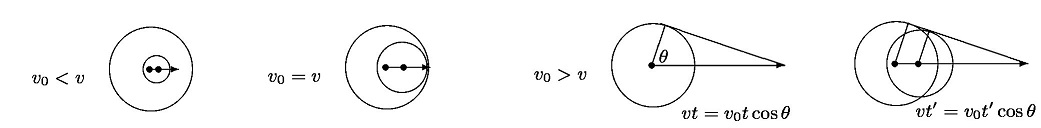
\includegraphics[width = \linewidth]{Cerenkov.jpg}
 \caption{Cerenkov 辐射示意图\label{fig:Cerenkov}}
\end{figure}
在 $\cos\theta = v/v_0$ 方向上会出现辐射场. 它是由于带电粒子超过介质中的光速时, 介质内产生诱导电流激发的次波与原来粒子的电磁场相互干涉形成的. 单位长度而非单位角的辐射强度是有限的
\begin{align}
    &\frac{\dif W_\omega}{\dif\Omega\dif L} = \frac{\omega^2 e^2\mu}{8\pi^2 v}\left(1-\frac{v^2}{v_0^2}\right)\delta\left[\left(1-\frac{\uvec r\cdot\vec v_0}{v}\right)\frac\omega{v_0}\right] \\
    &\frac{\dif W_\omega}{\dif L} = \frac{\omega e^2\mu}{4\pi }\left(1-\frac{v^2}{v_0^2}\right)
\end{align}
\begin{itemize}
    \item $W_\omega$ 只在 $v(\omega)<v_0$ 所给出的频段有贡献
    \item 不同频率的电磁波辐射角不同, 用滤波器选择一定的频带可以通过 $\theta$ 角测定粒子速度
    \item 广泛应用于粒子计数器, 有效避免低速粒子干扰
\end{itemize}
% subsubsection cerenkov_radiation (end)
% subsection EMF_of_a_moving_particle (end)
\subsection{带电粒子的电磁场对粒子本身的反作用} % (fold)
\label{sub:self_interaction}
能量守恒的角度, 在非电磁力 $\vec F$ 作用下
\begin{equation}
    (\vec F - m\vec a)\cdot \dif\vec l = \dif W_{\mbox{自}} + \dif W_{\mbox{辐}}
\end{equation}
从均匀带电球的电子模型出发 $\rho = -3e/4\pi r_e^3$, 可以得到
\begin{equation}
    \vec F + \vec F_s = \left(m + \frac 1{3c^2}W_e'\frac{5+v^2/c^2}{(1-v^2/c^2)^{3/2}}\right)\vec a
\end{equation}
其中 $W_e' = 3e^2/(20\pi\varepsilon_0 r_0)$ 是电子自身的电场能, $\vec F_s = \mu_0 e^2\dot{\vec a}/6\pi c$ 是电磁辐射的反冲. 略去相对论效应, 
\begin{equation}
    \vec F + \vec F_s = \left(m + \frac 5{3c^2}W_e'\right)\vec a
\end{equation}
其中 $m_e = m + 5W_e'/3c^2$ 是静止电子的电场能在运动起来时对质量的贡献, 称电磁质量. 加入认为电子质量主要来自于电磁质量, 那么
\begin{equation}
    r_e = \frac{\mu_0 e^2}{4\pi m_e} = 2.817\times 10^{-15}\mathrm m
\end{equation}

考虑辐射反冲力 $\vec F_s = \mu_0 e^2\dot{\vec a}/6\pi c$ 的形式会导致无限加速. 这是由于辐射反冲力的推导中要求周期性边界条件, 公式是周期性下的平均结果. 对于无限加速的情形并不满足周期性要求

\subsubsection{半经典发光模型} % (fold)
\label{ssub:semi_cla_light_emit}
电子均匀分布于原子内, 原子核处于电子云中心位置, 受到外界激发后原子核偏离电子云中心 $\vec r(t)$, 产生恢复力
\begin{equation}
    \vec F = -\frac{e\rho\vec r(t)}{3\varepsilon_0} \equiv -m_e\omega_0^2 r
\end{equation}
得到运动方程
\begin{equation}
    -m_e\omega_0^2 \vec r + \frac{\mu_0 e^2}{6\pi c}\dddot{\vec r} = m_e\ddot{\vec r}
\end{equation}
其中第二项为辐射反冲项. 试探解 $r = r_0\e^{-\mi\omega t}$, 得到
\begin{equation}
    \omega^2 = \omega_0^2 - \frac{\mi\mu_0 e^2}{6\pi c m_e}\omega^3 \qquad\Longrightarrow\qquad \omega\approx\omega_0 - \frac{\mi\mu_0 e^2\omega_0^2}{12\pi cm_e}\equiv \omega_0 - \frac{\mi\Gamma}{2}
\end{equation}
近似处理辐射场
\begin{equation}
    \vec B = \frac{e\mu_0}{4\pi cr}\vec a\times\uvec n, \qquad
    \vec E = c\vec B\times \uvec n
\end{equation}
做频谱分析的结果
\begin{equation}
    I_{\omega'} = \frac{c\varepsilon_0|E(r,0)|^2}{4\pi\left[(\omega'-\omega_0)^2 + \Gamma^2/4\right]}
\end{equation}
频谱宽度与频率无关
\begin{equation}
    \Delta\lambda = \frac{2\pi c}{\omega_0^2}\Delta\Gamma = \frac{\mu_0 e^2}{3m_e}\sim 10^{-4}\mbox{\AA}
\end{equation}
% subsubsection semi_cla_light_emit (end)
% subsection self_interaction (end)
\subsection{电磁波的散射与色散} % (fold)
\label{sub:scattering_and_dispersion}
\subsubsection{自由电子对电磁波的散射} % (fold)
\label{ssub:free_electro_scattering}
一定频率的外电磁波投射到电子上使电子以相同频率做受迫振动并向外辐射电磁波. 讨论电子速度 $v\ll c$, 电子线度和振幅 $l\ll\lambda$ 的情形, 并且忽略磁力
\begin{equation}
    m\ddot r = \frac{\mu_0 e^2}{6\pi c}\dddot r + e\vec E_0\e^{-\mi\omega t}
\end{equation}
试探解 $\vec r = r_0\e^{-\mi\omega t}$, 代入解得
\begin{equation}
    \vec r_0 = \frac{-e\vec E_0}{m\omega^2 - \mi\mu_0 e^2\omega^3/6\pi c}\approx -\frac{e\vec E_0}{m\omega^2}
\end{equation}
从而有散射波的电场和能流密度
\begin{align}
    &\vec E_r = \frac{e\mu_0\omega^2}{4\pi r}\left[\vec r_0 - (\uvec n\cdot\vec r_0)\uvec n\right]\e^{-\mi\omega(t-r/c)} \\
    &\overline{\vec S} = \frac12 \varepsilon_0c|E_r|^2\uvec n = \frac{\mu_0 e^4 E_0^2\sin^2\theta}{32\pi^2m_e^2 r^2 c}\uvec n = I_0\frac{r_e^2}{r^2}
\end{align}
其中 $\theta$ 是 $\vec E_0$ 与 $\uvec n$ 的夹角, 其中 $I_0 = E_0^2/2\mu_0 c$, $r_e = \mu_0 e^2/4\pi m_e$, 总的辐射强度
\begin{equation}
    I = \oint\dif\vec\sigma\cdot\vec S = \frac 83 \pi r_e^2 I_0\equiv\sigma I_0
\end{equation}
其中 $\sigma = 8\pi r_e^2/3$ 是 Thomson 散射截面
% subsubsection free_electro_scattering (end)
\subsubsection{束缚电子对电磁波的散射} % (fold)
\label{ssub:bounded_electro_scattering}
在运动方程中加入黏滞力项 $-\tilde{\gamma}\dot{\vec r}$
\begin{equation}
    m\ddot{\vec r} = -m\tilde{\gamma}\dot{\vec r} - \omega_0^2 m\vec r + e\vec E_0\e^{-\mi\omega t}
\end{equation}
试探解 $r = r_0\e^{-\omega t}$
\begin{equation}\label{equ:bounded_scattering}
    r_0 = \frac{e\vec E_0}{(\omega_0^2 - \omega^2)m - \mi\omega m\tilde{\gamma}}
    =\frac{e\vec E_0\e^{\mi\delta}}{m\sqrt{(\omega_0 - \omega^2)^2 + \omega^2\tilde{\gamma}^2} }
\end{equation}
散射能流
\begin{equation}
    \overline{\vec S} = I_0\frac{r_e^2}{r^2}\uvec n\sin^2\theta\frac{\omega^4}{(\omega_0^2 - \omega^2)^2 + \omega^2\tilde{\gamma}^2}
\end{equation}
\begin{itemize}
    \item Rayleigh 散射: 在 $\omega\ll\omega_0$ 时, $I\sim (\omega/\omega_0)^4$ \\
    可见光谱中, 红光散射最少, 紫光散射最多. 因而偏离入射方向时高频 (蓝) 光比重增加, 如天空蓝色
    \item $\omega\gg\omega_0$ 时, 退化为自由电子的情形
\end{itemize}
% subsubsection bounded_electro_scattering (end)
\subsubsection{介质的色散} % (fold)
\label{ssub:medium_scattering}
介质中单位体积电子数 $N$, 固有频率均为 $\omega$, 极化强度 $\vec P = \varepsilon_0\chi_e \vec E = Ne \vec r$, 则引用式(\ref{equ:bounded_scattering}) 得到
\begin{equation}
    \chi_e = \frac{Ne^2}{m\varepsilon_0(\omega_0^-\omega^2 - \mi\omega\tilde{\gamma})}
\end{equation}
而 $\varepsilon = \varepsilon_0(1+\chi_e)$ 具有虚部表示电导, 造成电磁波的吸收. 实部与 $\omega$ 有关造成不同频率波的折射率不同, 导致色散.

如略去衰减, 在 $\omega\ll\omega_0$ 的近似下, 讨论折射角和频率的关系
\begin{equation}
    \delta\varepsilon \approx (\varepsilon - \varepsilon_0)\frac{\delta\omega^2}{\omega_0^2}, \qquad \delta\theta = -\frac{(\varepsilon_r - 1)\omega}{\omega_0^2\varepsilon_r}\tan\theta\delta\omega
\end{equation}
可见频率小的偏转角度大. 解释彩虹红光偏转角最大, 相当于像在最高位置, 紫光反之. 霓因为多一次反射, 折射角和偏转角关系恰反之.

一般当 $\omega\neq 0 $ 时, 都具有一定的导电性. 讨论黏滞系数, 则会出现特定的吸收峰值.
% subsubsection medium_scattering (end)
\subsubsection{电磁感应透明} % (fold)
\label{ssub:EM_transparency}
考虑介质具有特殊的隐自由度 $\vec\xi(t)$
\begin{equation}
    m\ddot{\vec r} = -m\tilde\gamma\dot{\vec r} - \omega_0^2 m\vec r + \Omega m\vec\xi + e\vec E_0\e^{-\mi\omega t},\qquad m\ddot{\vec \xi} = -\omega_0^2 m\vec \xi + \Omega m\vec r
\end{equation}
类似上面的解法可以得到
\begin{equation}
    \chi_e = \frac{Ne^2}{\varepsilon_0 m}\frac{(\omega_0^2 - \omega^2)}{(\omega_0^2 - \omega^2)(\omega_0^2 - \omega^2 - \mi\omega\tilde\gamma)-\Omega^4}
\end{equation}
当 $\omega\to\omega_0$ 时, 出现 $\chi_e\to 0$, 表现为电磁感应透明
% subsubsection EM_transparency (end)
\subsubsection{因果性与色散关系} % (fold)
\label{ssub:causality}
一般的研究线性介质极化率与电磁波频率的关系, 考虑历史
\begin{equation}
    \vec P(\vec r,t) =\int_0^\infty\dif t' f(t')\vec E(\vec r,t-t')
\end{equation}
因果性要求 $t$ 时刻之后的 $\vec E$ 对于 $\vec P(t)$ 无影响, 因而上的积分下限取 $0$, 于是
\begin{equation}
    \chi_e(\omega) = \int_0^\infty\dif t\e^{\mi\omega t}f(t) = \chi^*_e(-\omega)
\end{equation}
再加上越早的 $\vec E$ 对 $\vec P$ 影响越小, 即 $\lim_{t\to\infty} f(t) = 0$, 于是得知 $\chi_e(\omega)$ 在 $\omega$ 的上半复平面上存在且解析, 且 $\lim_{\omega\to\infty}\chi_e(\omega) = 0$. 从而由解析性, $\chi_e$ 的实部和虚部相联系.
% subsubsection causality (end)
% subsection scattering_and_dispersion (end)
% section elec_partic_and_field (end)
\end{document}